\documentclass[UTF8]{ctexart}
\title{永磁同步电机:实验报告}
\author{1852479 康嘉梁}
\date{}
\ctexset{
bibname = {参考文献},
}
\pagestyle{plain}

\usepackage[a4paper]{geometry}
\geometry{left=3.18cm,right=3.18cm,top=2.54cm,bottom=2.54cm}

\usepackage[hidelinks]{hyperref}%为交叉引用添加链接的宏包

\usepackage{amsmath}
\numberwithin{figure}{section}
\numberwithin{table}{section}

% \renewcommand\thesection{\chinese{section}}
% \renewcommand\thesubsection{\arabic{subsection}}
% \renewcommand\thesubsubsection{\thesubsection\thinspace.\thinspace\arabic{subsubsection}}
\renewcommand\thesubsubsection{\alph{subsubsection})}

\usepackage[version=4]{mhchem}

\usepackage{siunitx}
\DeclareSIUnit\rpm{rpm}

\usepackage{cleveref}
\crefname{section}{节}{节}
\crefname{equation}{式}{式}
\crefname{figure}{图}{图}
\crefname{table}{表}{表}
\crefname{appendix}{附录}{附录}
\newcommand{\crefpairconjunction}{~和~}
\newcommand{\crefmiddleconjunction}{、}
\newcommand{\creflastconjunction}{~和~}
\newcommand{\crefpairgroupconjunction}{~和~}
\newcommand{\crefmiddlegroupconjunction}{、}
\newcommand{\creflastgroupconjunction}{~和~}
\newcommand{\crefrangeconjunction}{~}

\usepackage{graphicx}
\DeclareGraphicsExtensions{.eps,.jpg,.png}
\graphicspath{{img}}
\usepackage{caption}
\captionsetup[figure]{labelsep=period}
\usepackage{float} %设置图片浮动位置的宏包
\usepackage{subfigure} %插入多图时用子图显示的宏包

\begin{document}
\maketitle
\tableofcontents

\clearpage


\section{实验设置}

选用\SI{100}{\kilo\watt} PMSM电机,电机参数为:定子相电阻$R_s$=\SI{8.3}{\milli\ohm},定子匝链相绕组永磁磁链峰值$\psi_f$=\SI{0.071}{\weber},电机极对数$p$=4,转动惯量$J$=\SI{0.1}{\kilo\gram\cdot\metre\squared},定子绕组相漏电感$L_\sigma$=\SI{30}{\micro\henry},d轴励磁电感$L_{md}$=\SI{174}{\micro\henry},q轴励磁电感$L_{mq}$=\SI{293}{\micro\henry},额定转速$n$=\SI{4700}{\rpm},峰值转矩$t_{e\rm max}$=\SI[inter-unit-product=\ensuremath{\cdot}]{256}{\newton\metre}。
假设电机的最高转速为$n_{\rm max}$=\SI{12000}{\rpm}。

由以上数据可以求得,电机的直轴同步电感$L_d=L_\sigma+L_{md}$=\SI{204}{\micro\henry},交轴同步电感$L_q=L_\sigma+L_{mq}$=\SI{323}{\micro\henry}。


\section{实验内容}

\subsection{峰值转矩对应峰值相电流}
\label{subsection:2.1}

电机的恒转矩电流表达式\cite{b}为:
\begin{equation}
	i_q=\frac{2t_e}{3p[\psi_f+(L_d-L_q)i_d]}\label{constT}
\end{equation}

MTPA曲线\cite{b}为:
\begin{equation}
	i_q=\pm\sqrt{i_d\left(i_d+\frac{\psi_f}{L_d-L_q}\right)},\quad i_d<0\label{MTPA}
\end{equation}

将$t_{e\rm max}$=\SI[inter-unit-product=\ensuremath{\cdot}]{256}{\newton\metre}代入\cref{constT},并与\cref{MTPA}联立,求两曲线在II象限的交点,即为峰值$d$轴电流$i_{d\rm max}$=\SI[round-mode=places,round-precision=2]{-228.677222}{\ampere},峰值$q$轴电流$i_{q\rm max}$=\SI[round-mode=places,round-precision=2]{434.431746}{\ampere}。峰值电流$i_{s\rm max}=\sqrt{i_{d\rm max}^2+i_{q\rm max}^2}$=\SI[round-mode=places,round-precision=2]{490.9422}{\ampere}。

\subsection{恒转矩曲线(渐近线)、等转矩线}
\label{subsection:2.2}

不同转矩下的恒转矩曲线为一簇均以$i_d=\psi_f/(L_q-L_d)$和$i_q=0$为渐近线的双曲线,取正转矩的部分画出如\cref{constque}。

将II、III象限的等转矩曲线用虚线标出,各曲线上与原点距离最小点的连线即为\cref{MTPA}表示的MTPA曲线,如\cref{equtque}。

\begin{figure}[htbp]
	\centering
	\begin{minipage}[b]{0.8\textwidth}
		\centering
		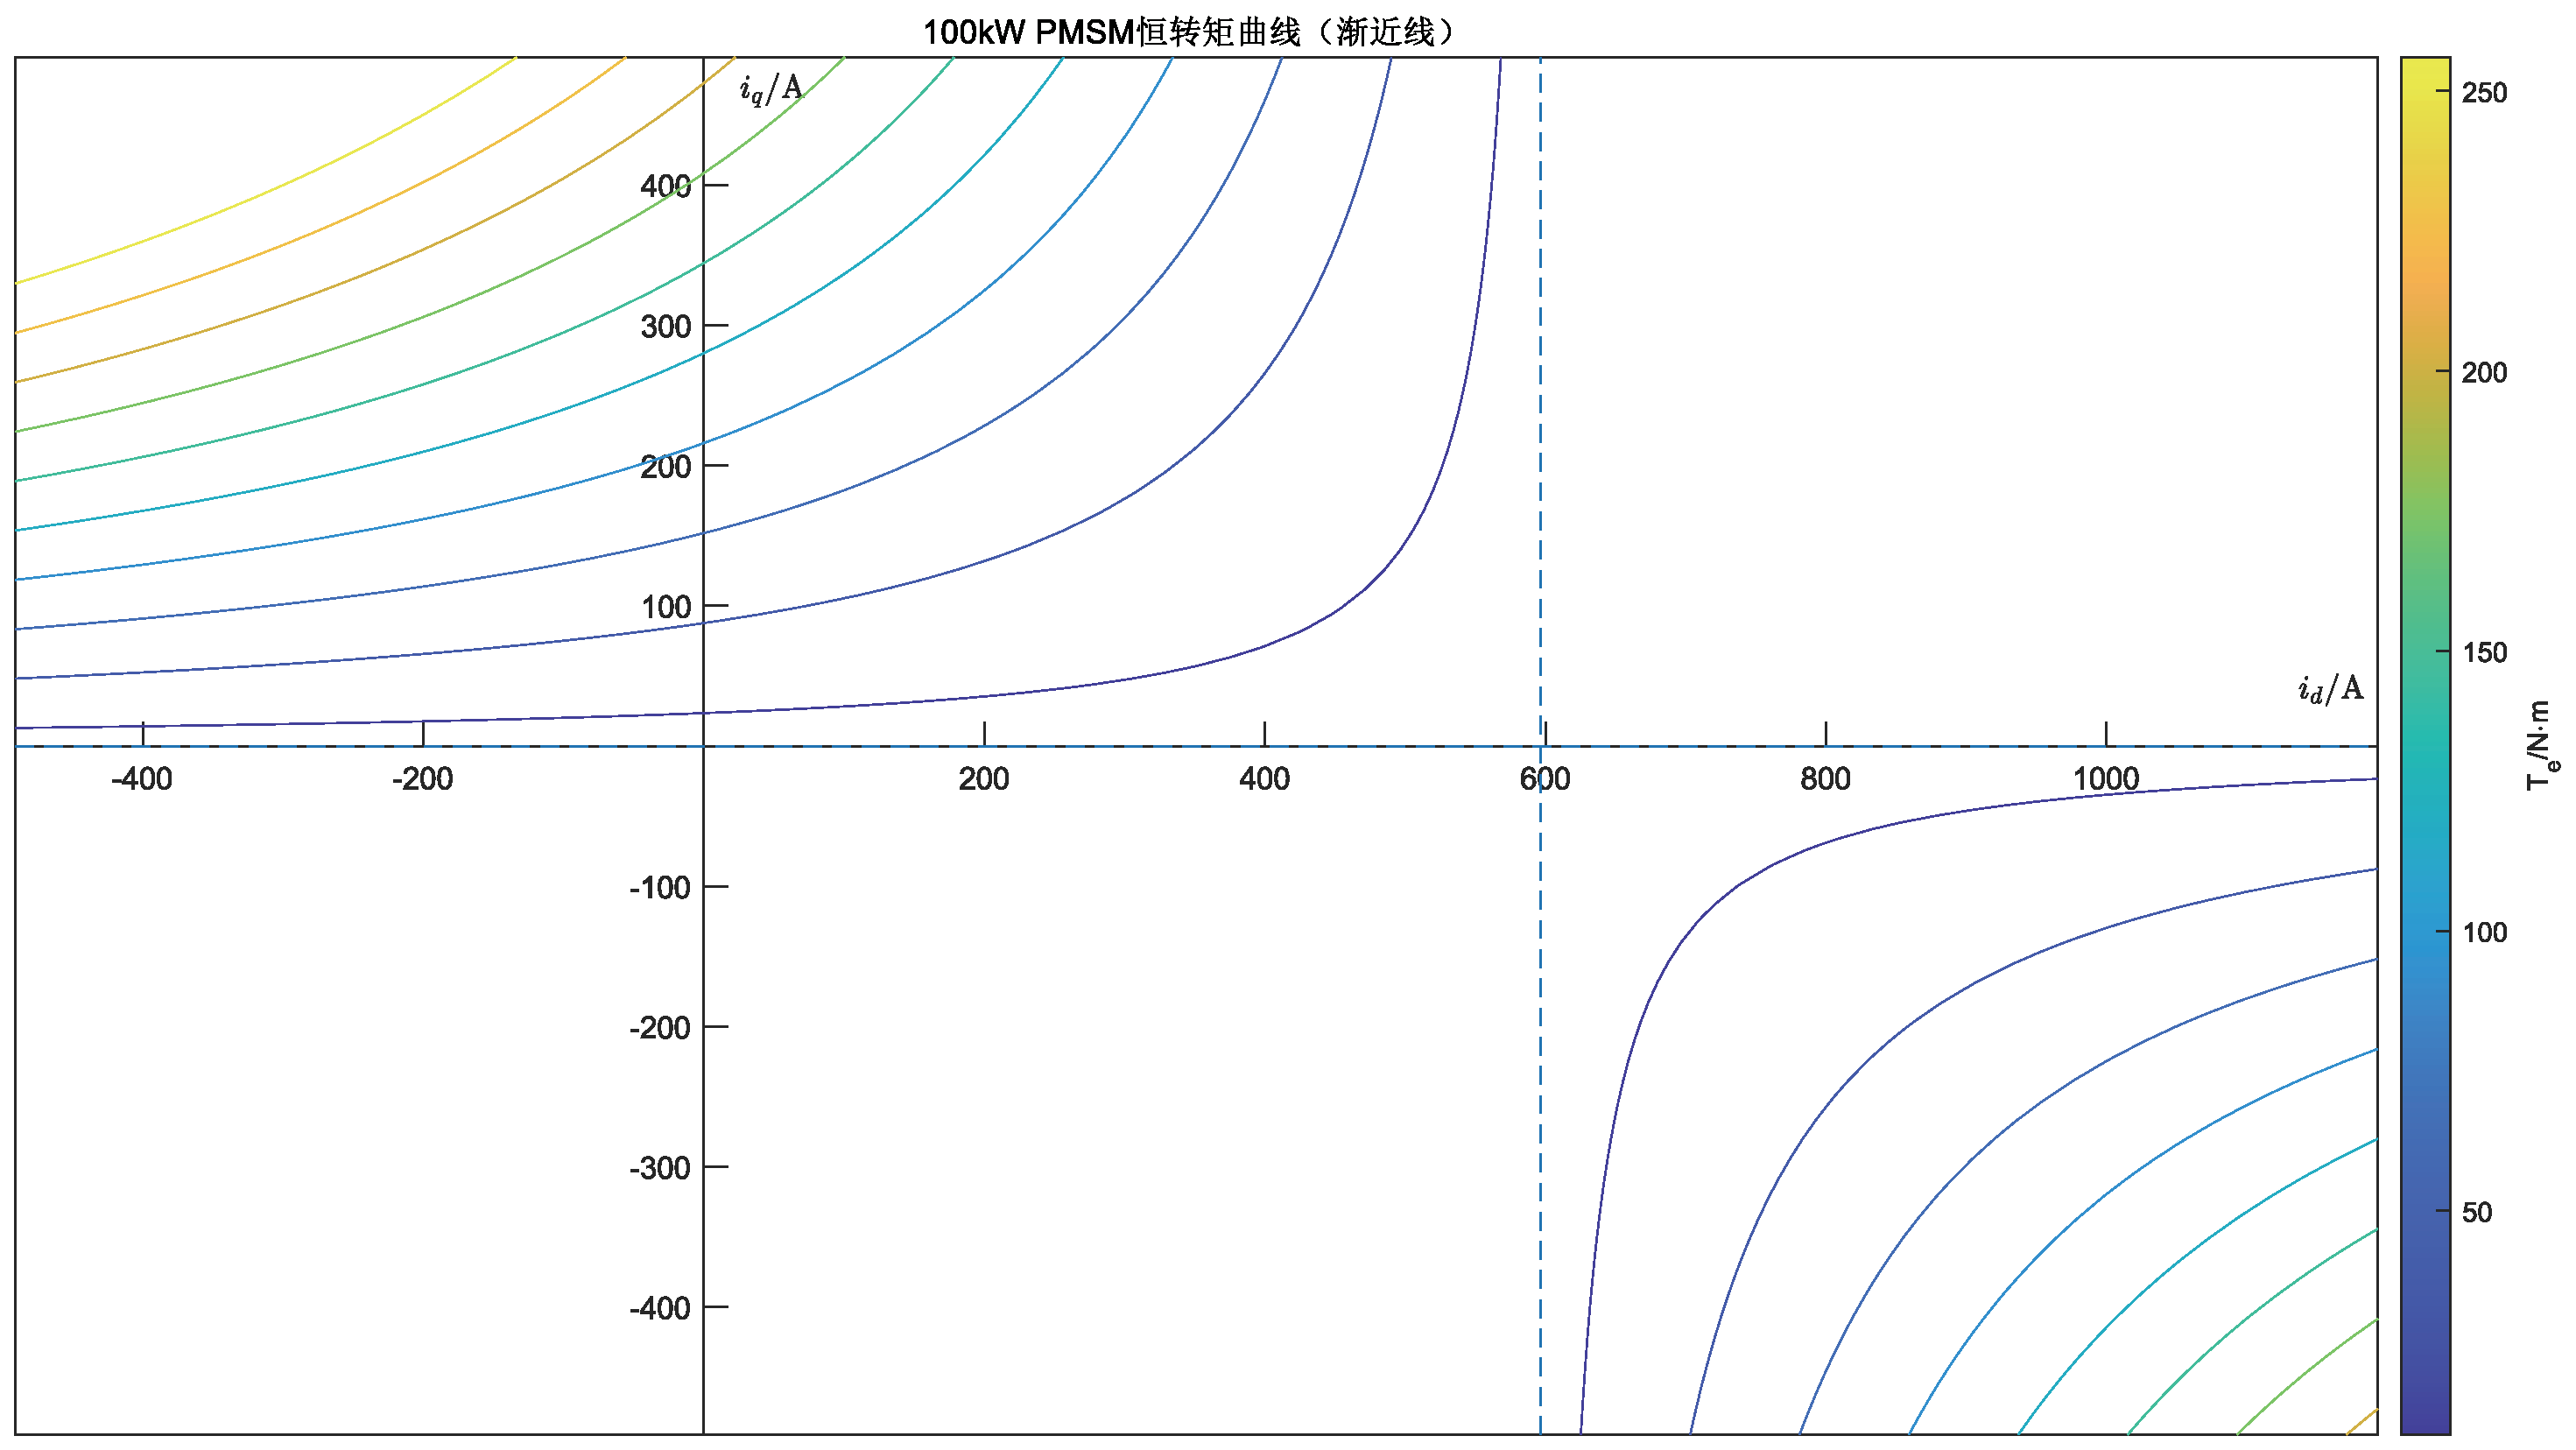
\includegraphics[width=\textwidth]{1}
		\caption{恒转矩曲线(渐近线)}
		\label{constque}
	\end{minipage}
	\begin{minipage}[b]{0.8\textwidth}
		\centering
		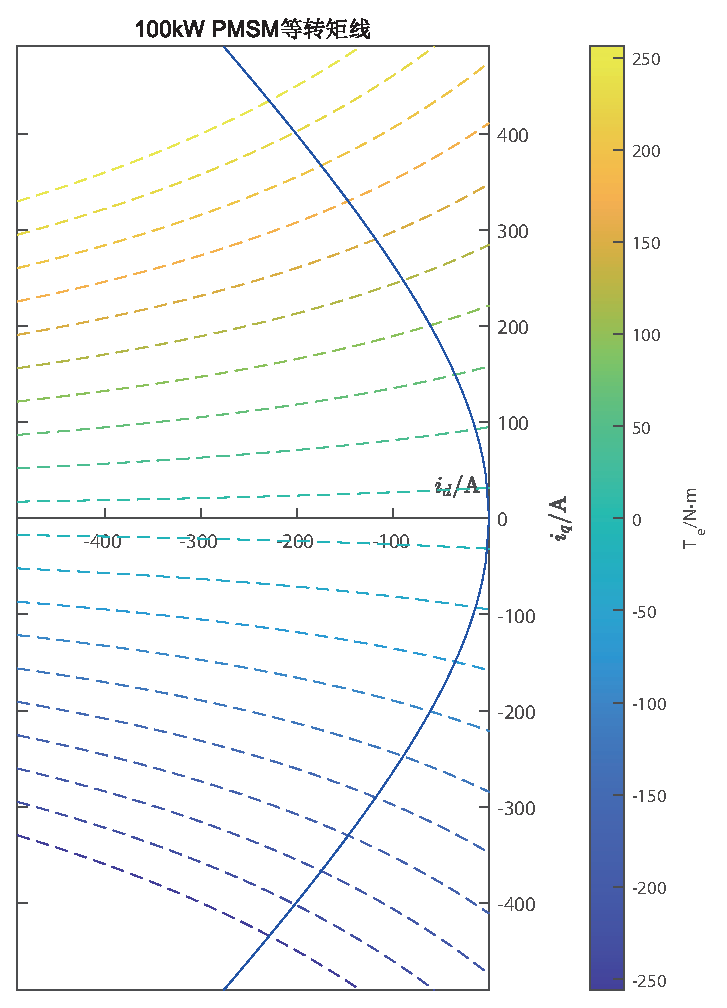
\includegraphics[width=\textwidth]{2}
		\caption{等转矩线}
		\label{equtque}
	\end{minipage}
\end{figure}

\subsection{电压极限椭圆(簇)}
\label{subsection:2.3}

电机的基速\cite{b}:
\begin{equation}
	\omega_{rb}=\frac{2\pi n}{60p}\label{omega_rb}
\end{equation}
代入额定转速$n$=\SI{4700}{\rpm},电机极对数$p$=4,求得$\omega_{rb}$=\SI[round-mode=places,round-precision=2,inter-unit-product=\ensuremath{\cdot}]{1.9687e+03}{\radian\per\second}。

类似地,电机最高速度$\omega_{r\rm max}=(2\pi n_{\rm max}/60p)$=\SI[round-mode=places,round-precision=2,inter-unit-product=\ensuremath{\cdot}]{5.0265e+03}{\radian\per\second}。

通过\cref{Usm}\cite{b}:
\begin{equation}
	U_{sm}=\omega_{rb}\sqrt{(L_di_{d\rm max}+\psi_f)^2+(L_qi_{q\rm max})^2}\label{Usm}
\end{equation}
可求得峰值电压$U_{sm}$=\SI[round-mode=places,round-precision=2]{280.3837}{\volt}。

电压极限椭圆簇\cite{b}为:
\begin{equation}
	(L_di_d+\psi_f)^2+(L_qi_q)^2=\left(\frac{U_{sm}}{\omega_r}\right)^2\label{voltLim}
\end{equation}

电流极限圆\cite{b}为:
\begin{equation}
	i_d^2+i_q^2=i_{s\rm max}^2\label{curLim}
\end{equation}

取电压极限椭圆簇中转子速度在$\omega_{rb}$和$\omega_{r\rm max}$之间的部分用虚线画出,同时用实线画出电流极限圆,如\cref{voltLimFig}。

\begin{figure}[htbp]
	\centering
	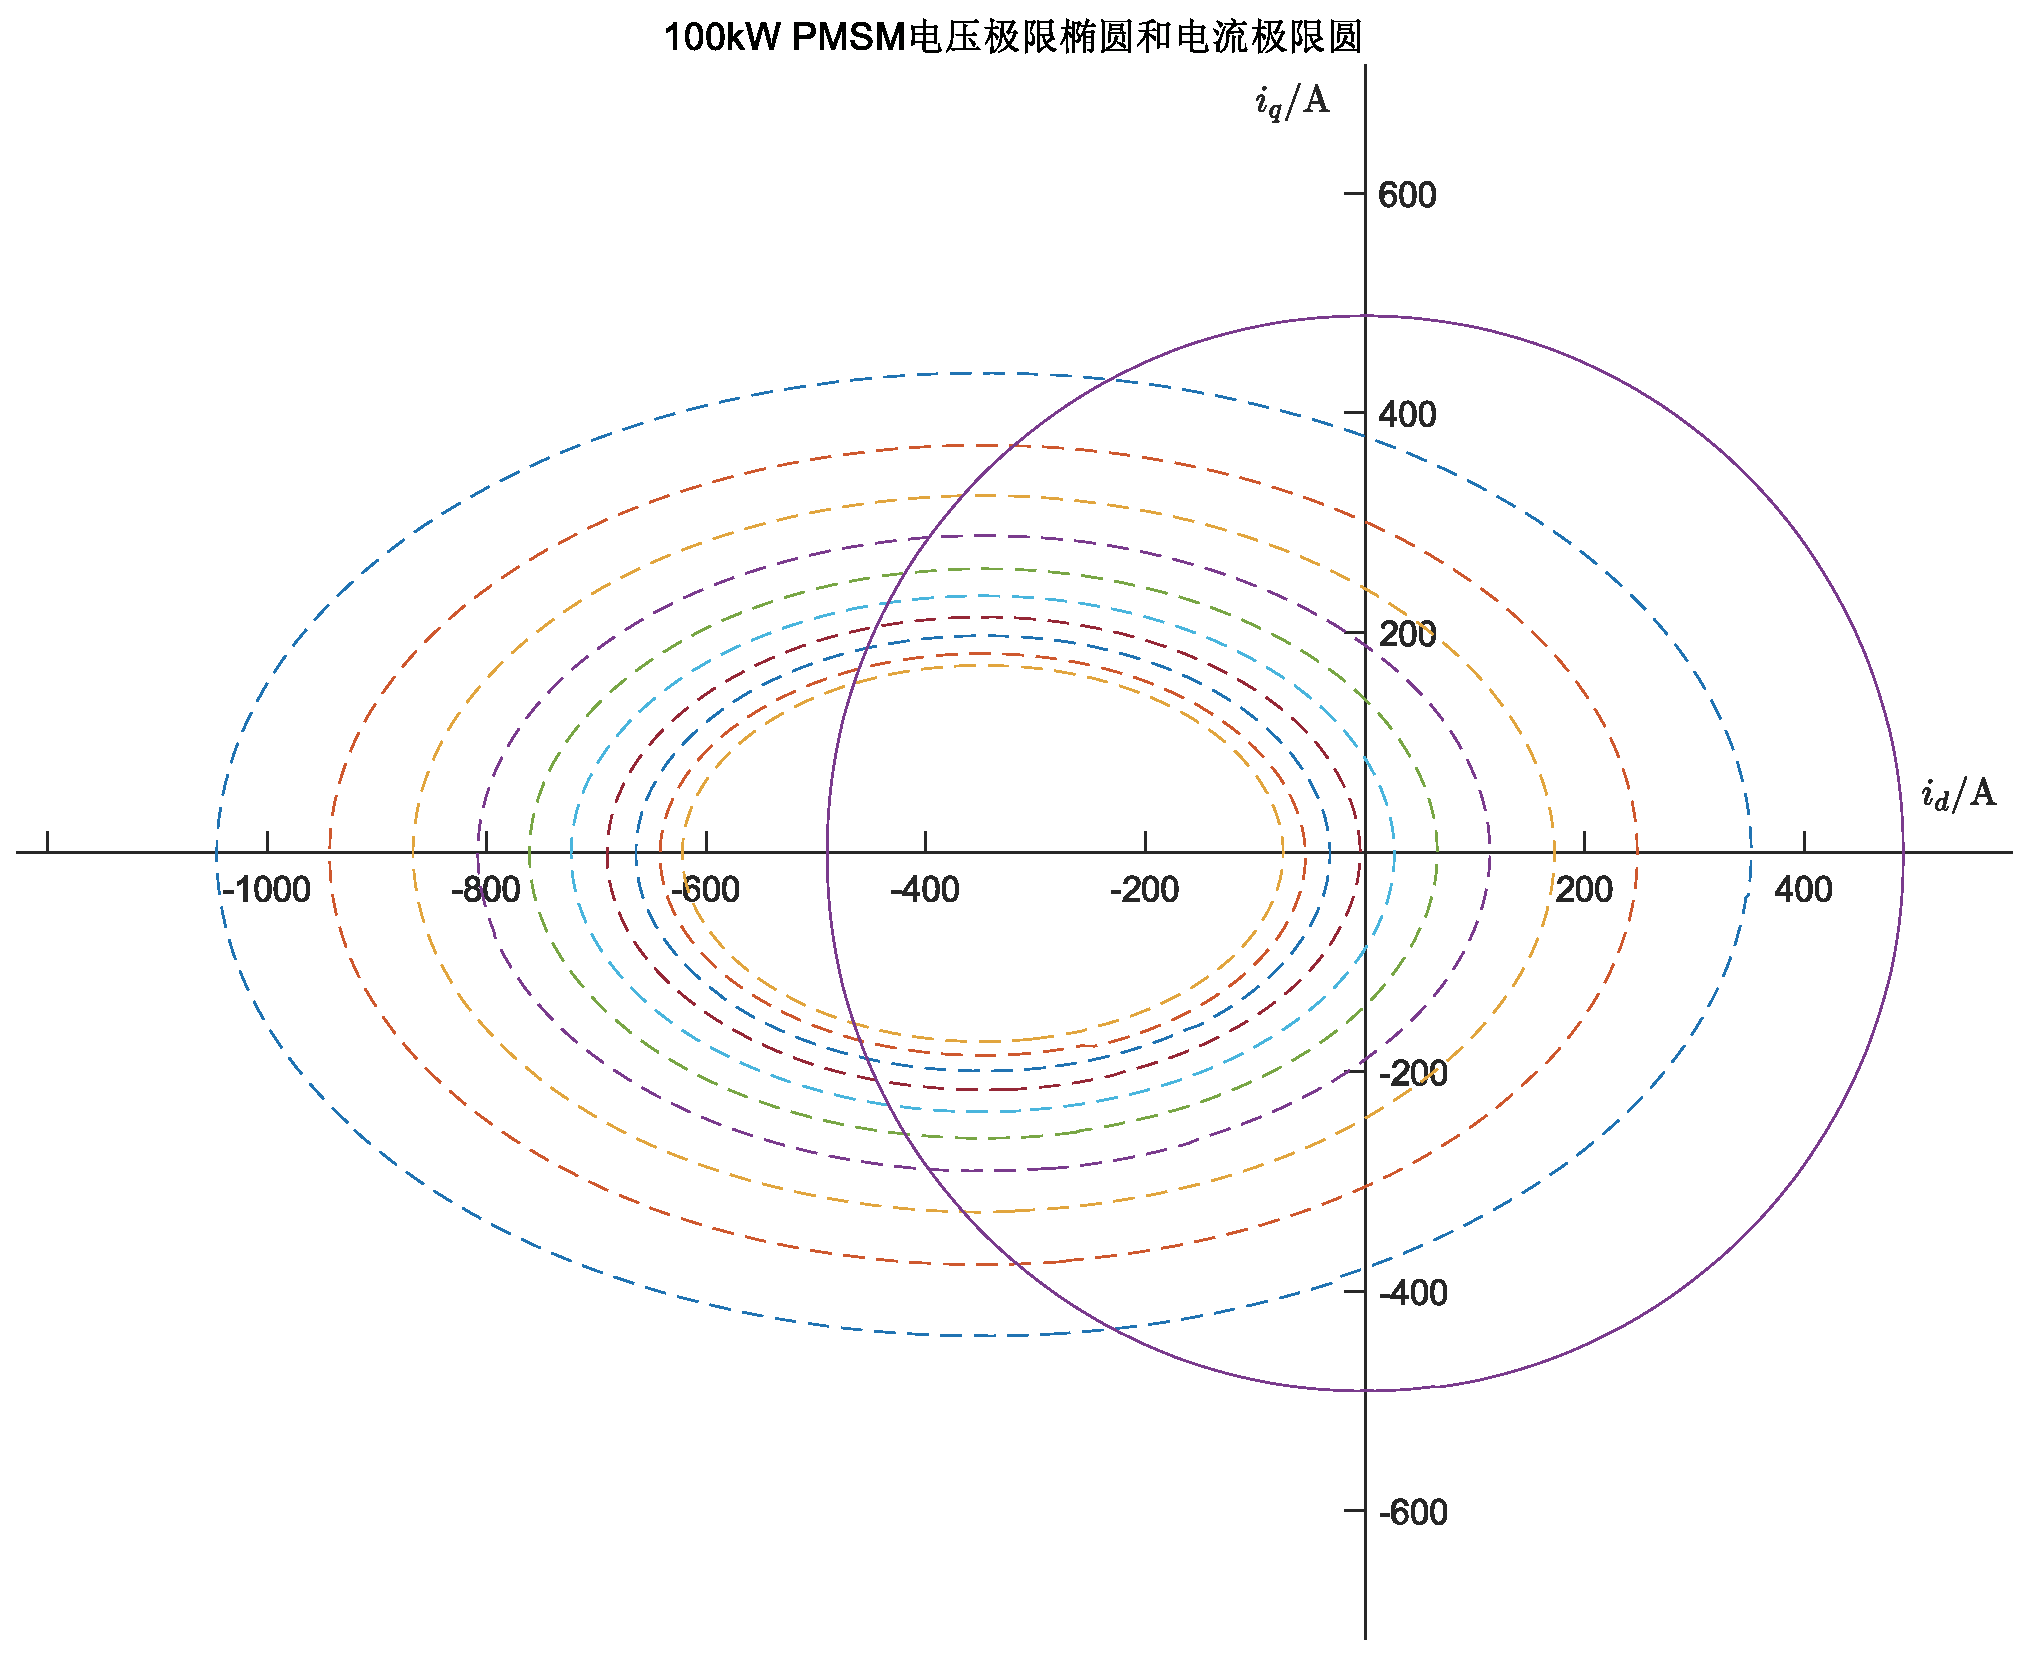
\includegraphics[width=0.8\textwidth]{3}
	\caption{电压极限椭圆(簇)}
	\label{voltLimFig}
\end{figure}

\subsection{最大转矩电流比(MTPA)曲线}
\label{subsection:2.4}

MTPA曲线的公式如\cref{MTPA},为最小定子电流矢量轨迹\cite{b}。

\subsection{最大转矩电压比(MTPV)曲线}
\label{subsection:2.5}

MTPV曲线的公式\cite{b}为:
\begin{equation}
	i_q=\pm\sqrt{\frac{L_d(L_di_d+\psi_f)[(L_d-L_q)i_d+\psi_f]}{(L_d-L_q)L_q^2}},\quad i_d<-\frac{\psi_f}{L_d}\label{MTPV}
\end{equation}
其上的每一点都表示了在给定电压下能达到的转速$\omega_r$的最大值。

MTPA曲线和MTPV曲线及电压极限椭圆和电流极限椭圆同时画在\cref{MTPA and MTPV}中。

\begin{figure}[htbp]
	\centering
	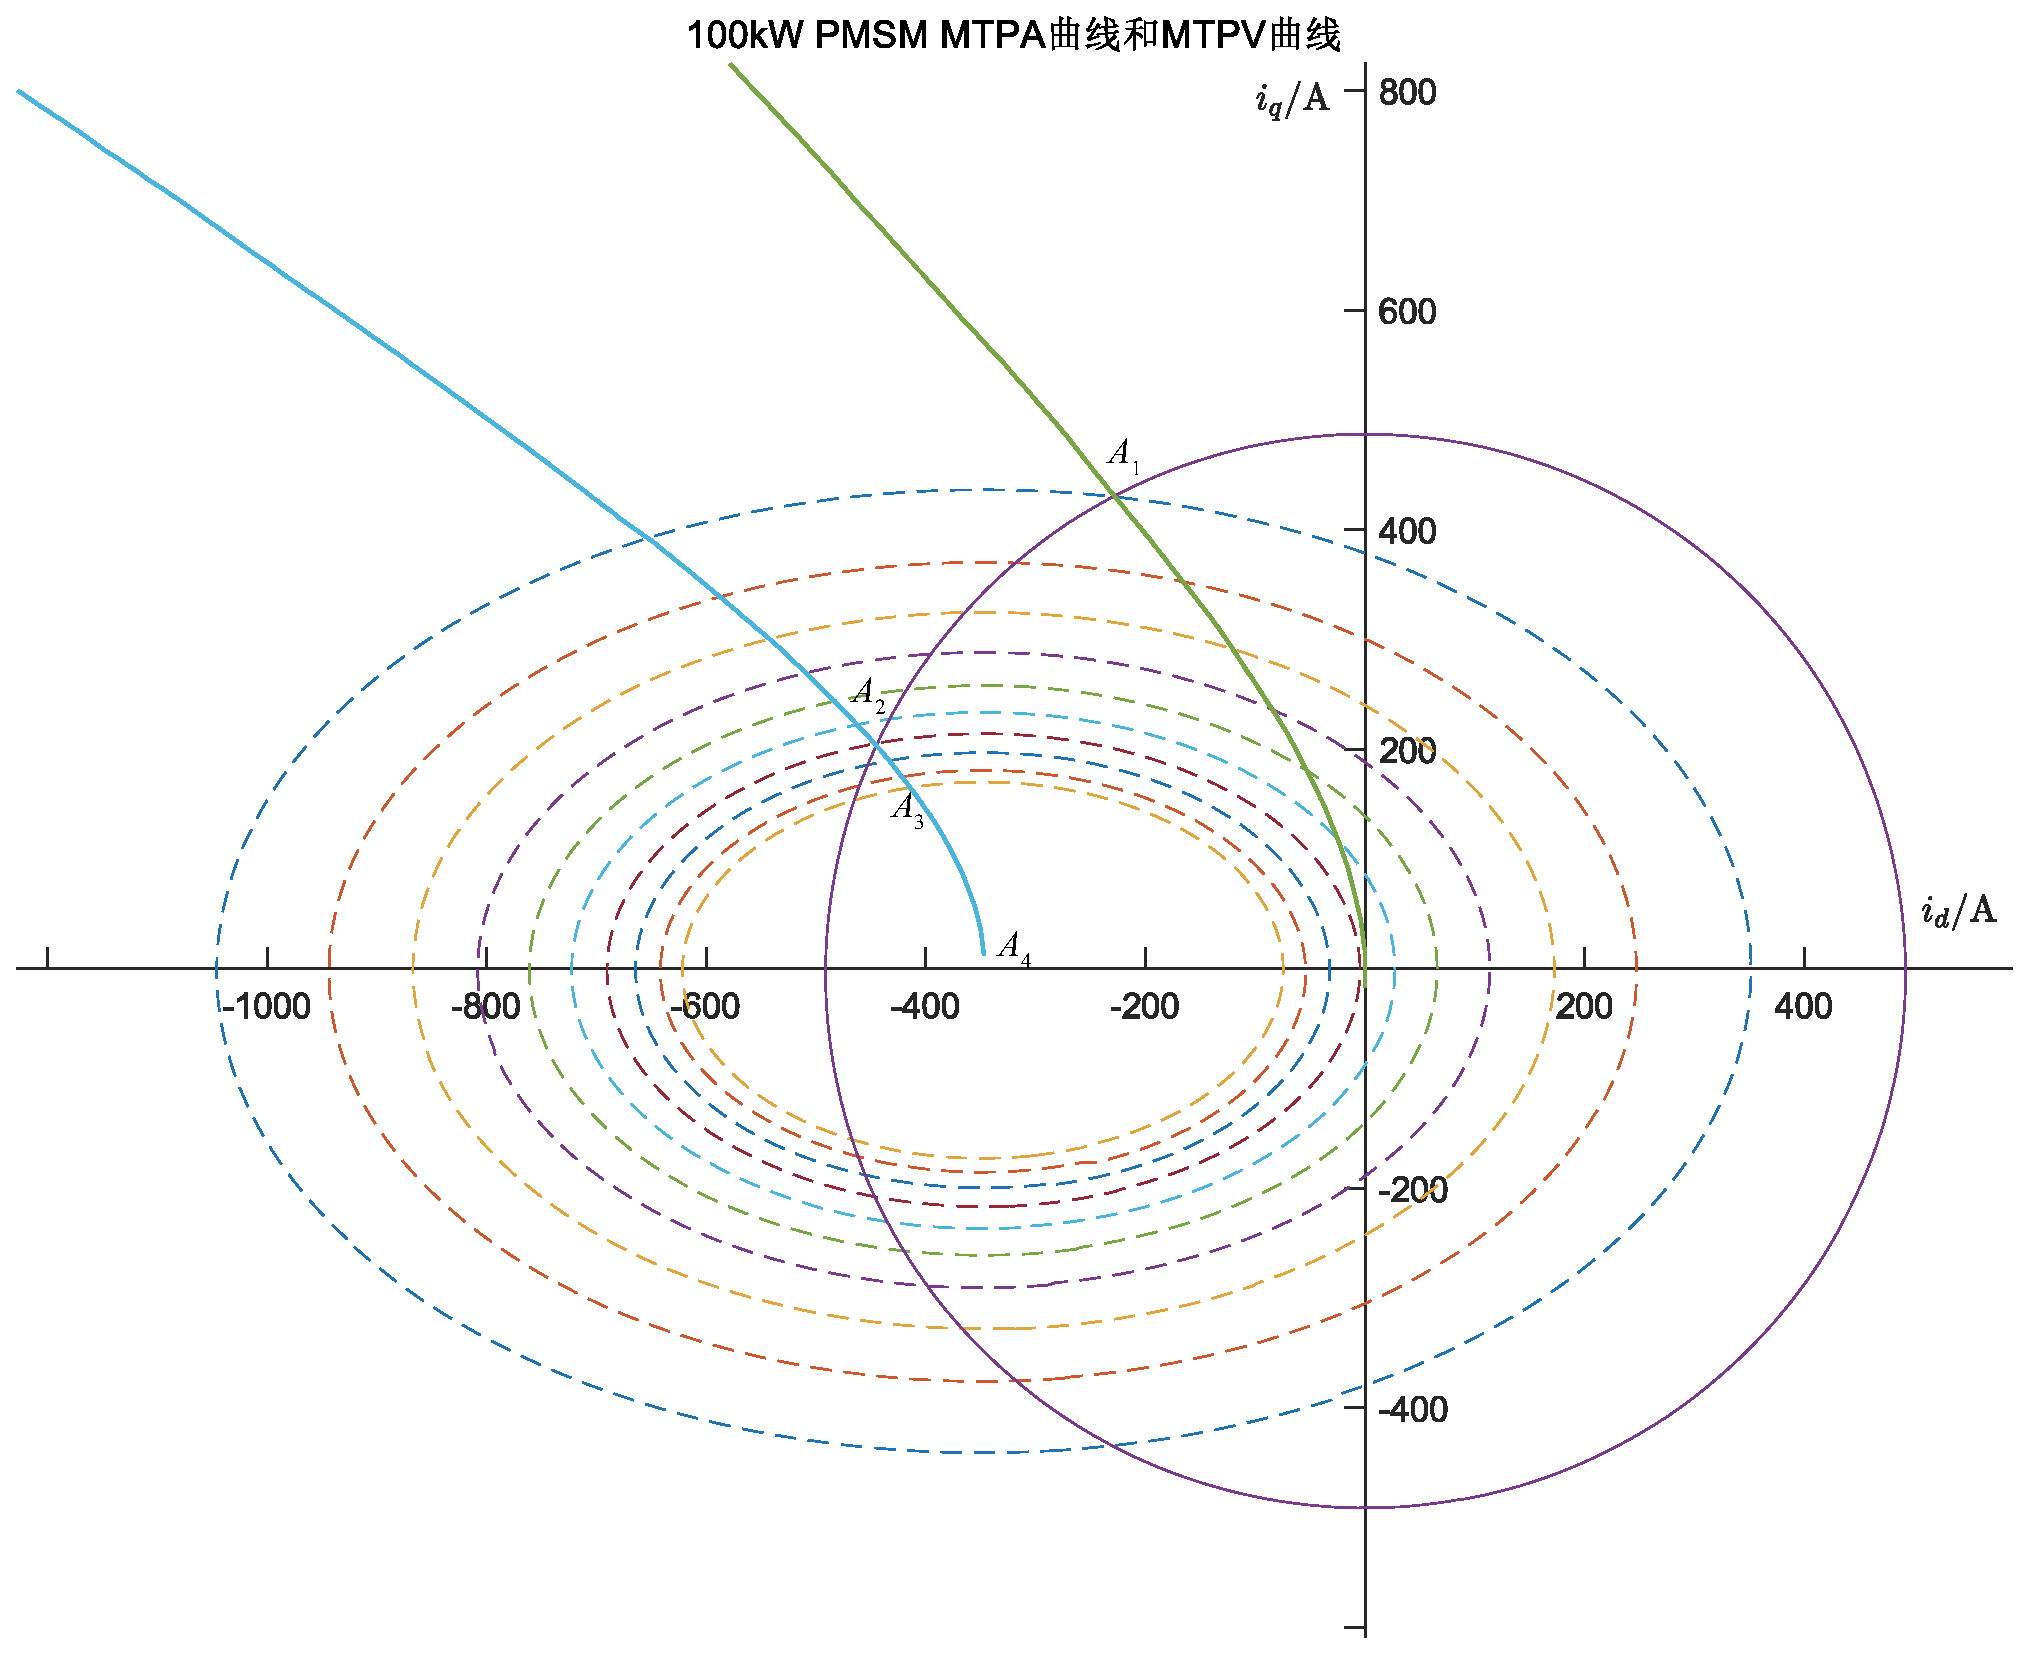
\includegraphics[width=0.8\textwidth]{4}
	\caption{MTPA曲线和MTPV曲线}
	\label{MTPA and MTPV}
\end{figure}

\subsection{机械特性(外特性)}
\label{subsection:2.6}

对于该电机,由\cref{MTPA and MTPV}可知,$A_4$点在电流极限圆内部,即$\psi_f/L_d<i_{s\rm max}$,电机可以实现最大功率输出控制。已知$A_1$、$A_3$点转子速度分别为基速$\omega_{rb}$和最大速度$\omega_{r\rm max}$,设$A_2$点转子速度为$\omega_{r2}$。控制策略随转速的增加依次划分为恒转矩区($0\le\omega_r\le\omega_{rb}$)、弱磁I区($\omega_{rb}<\omega_r\le\omega_{r2}$)和弱磁II区($\omega_r>\omega_{r2}$)。

对任意工作点,电机输出的转矩$t_e$和功率$P_e$、输入的电压$u_s$和电流$i_s$均可表示为$d$轴电流$i_d$、$q$轴电流$i_q$和转子的电角速度$\omega_r$的函数,如\cref{Te,Pe,Us,Is}\cite{b}:
\begin{align}
	t_e(i_d,i_q)          & =\frac{3}{2}p[\psi_fi_q+(L_d-L_q)i_di_q] \label{Te}                    \\
	P_e(i_d,i_q,\omega_r) & =\frac{3}{2}\omega_r[\psi_fi_q+(L_d-L_q)i_di_q] \label{Pe}             \\
	u_s(i_d,i_q,\omega_r) & =\sqrt{(\omega_rL_di_d+\omega_r\psi_f)^2+(\omega_rL_qi_q)^2}\label{Us} \\
	i_s(i_d,i_q)          & =\sqrt{i_d^2+i_q^2}\label{Is}
\end{align}
其中\cref{Us}忽略了铜损。


可见,我们仅需找出每个转子速度$\omega_r$下需控制的$d$轴电流$i_d$和$q$轴电流$i_q$,即可绘制出电机的外特性曲线。

恒转矩区($0\le\omega_r\le\omega_{rb}$)的全部工作点均对应\cref{MTPA and MTPV}中的$A_1$点,故该区内恒有:
\begin{align}
	i_d & =i_{d\rm max} \\
	i_q & =i_{q\rm max}
\end{align}
其中$i_{d\rm max}$和$i_{q\rm max}$在$\cref{subsection:2.1}$中给出,注意下标``$_{\rm max}$"并非表示$i_d$和$i_q$均取得最大值,仅表示电流为峰值转矩对应的电流。

在弱磁I区($\omega_{rb}<\omega_r\le\omega_{r2}$),电压和电流同时饱和,定子电流矢量沿电流极限圆的圆周从$A_1$点向$A_2$点移动,$\omega_r$取电压限制下的最大值。$i_d$、$i_q$可由电流极限圆方程(\cref{curLim})和各$\omega_r$对应的电压极限椭圆方程(\cref{voltLim})联立求解。

在弱磁II区($\omega_r>\omega_{r2}$),定子电流矢量沿最大功率输出轨迹,即MTPV线,从$A_2$点向$A_4$点移动,直至$\omega_r$在$A_3$点处取到$\omega_{r\rm max}$。电压$u_s$保持饱和,故$i_d$、$i_q$可由MTPV方程(\cref{MTPV})和各$\omega_r$对应的电压极限椭圆方程(\cref{voltLim})联立求解。

这样,外特性曲线上每个转子速度$\omega_r$下对应的$i_d$、$i_q$均已求得,把他们代入\cref{Te,Pe,Us,Is},并按习惯将横坐标转换回转速,即可画出外特性曲线如\cref{extChar}。

\begin{figure}[htbp]
	\centering
	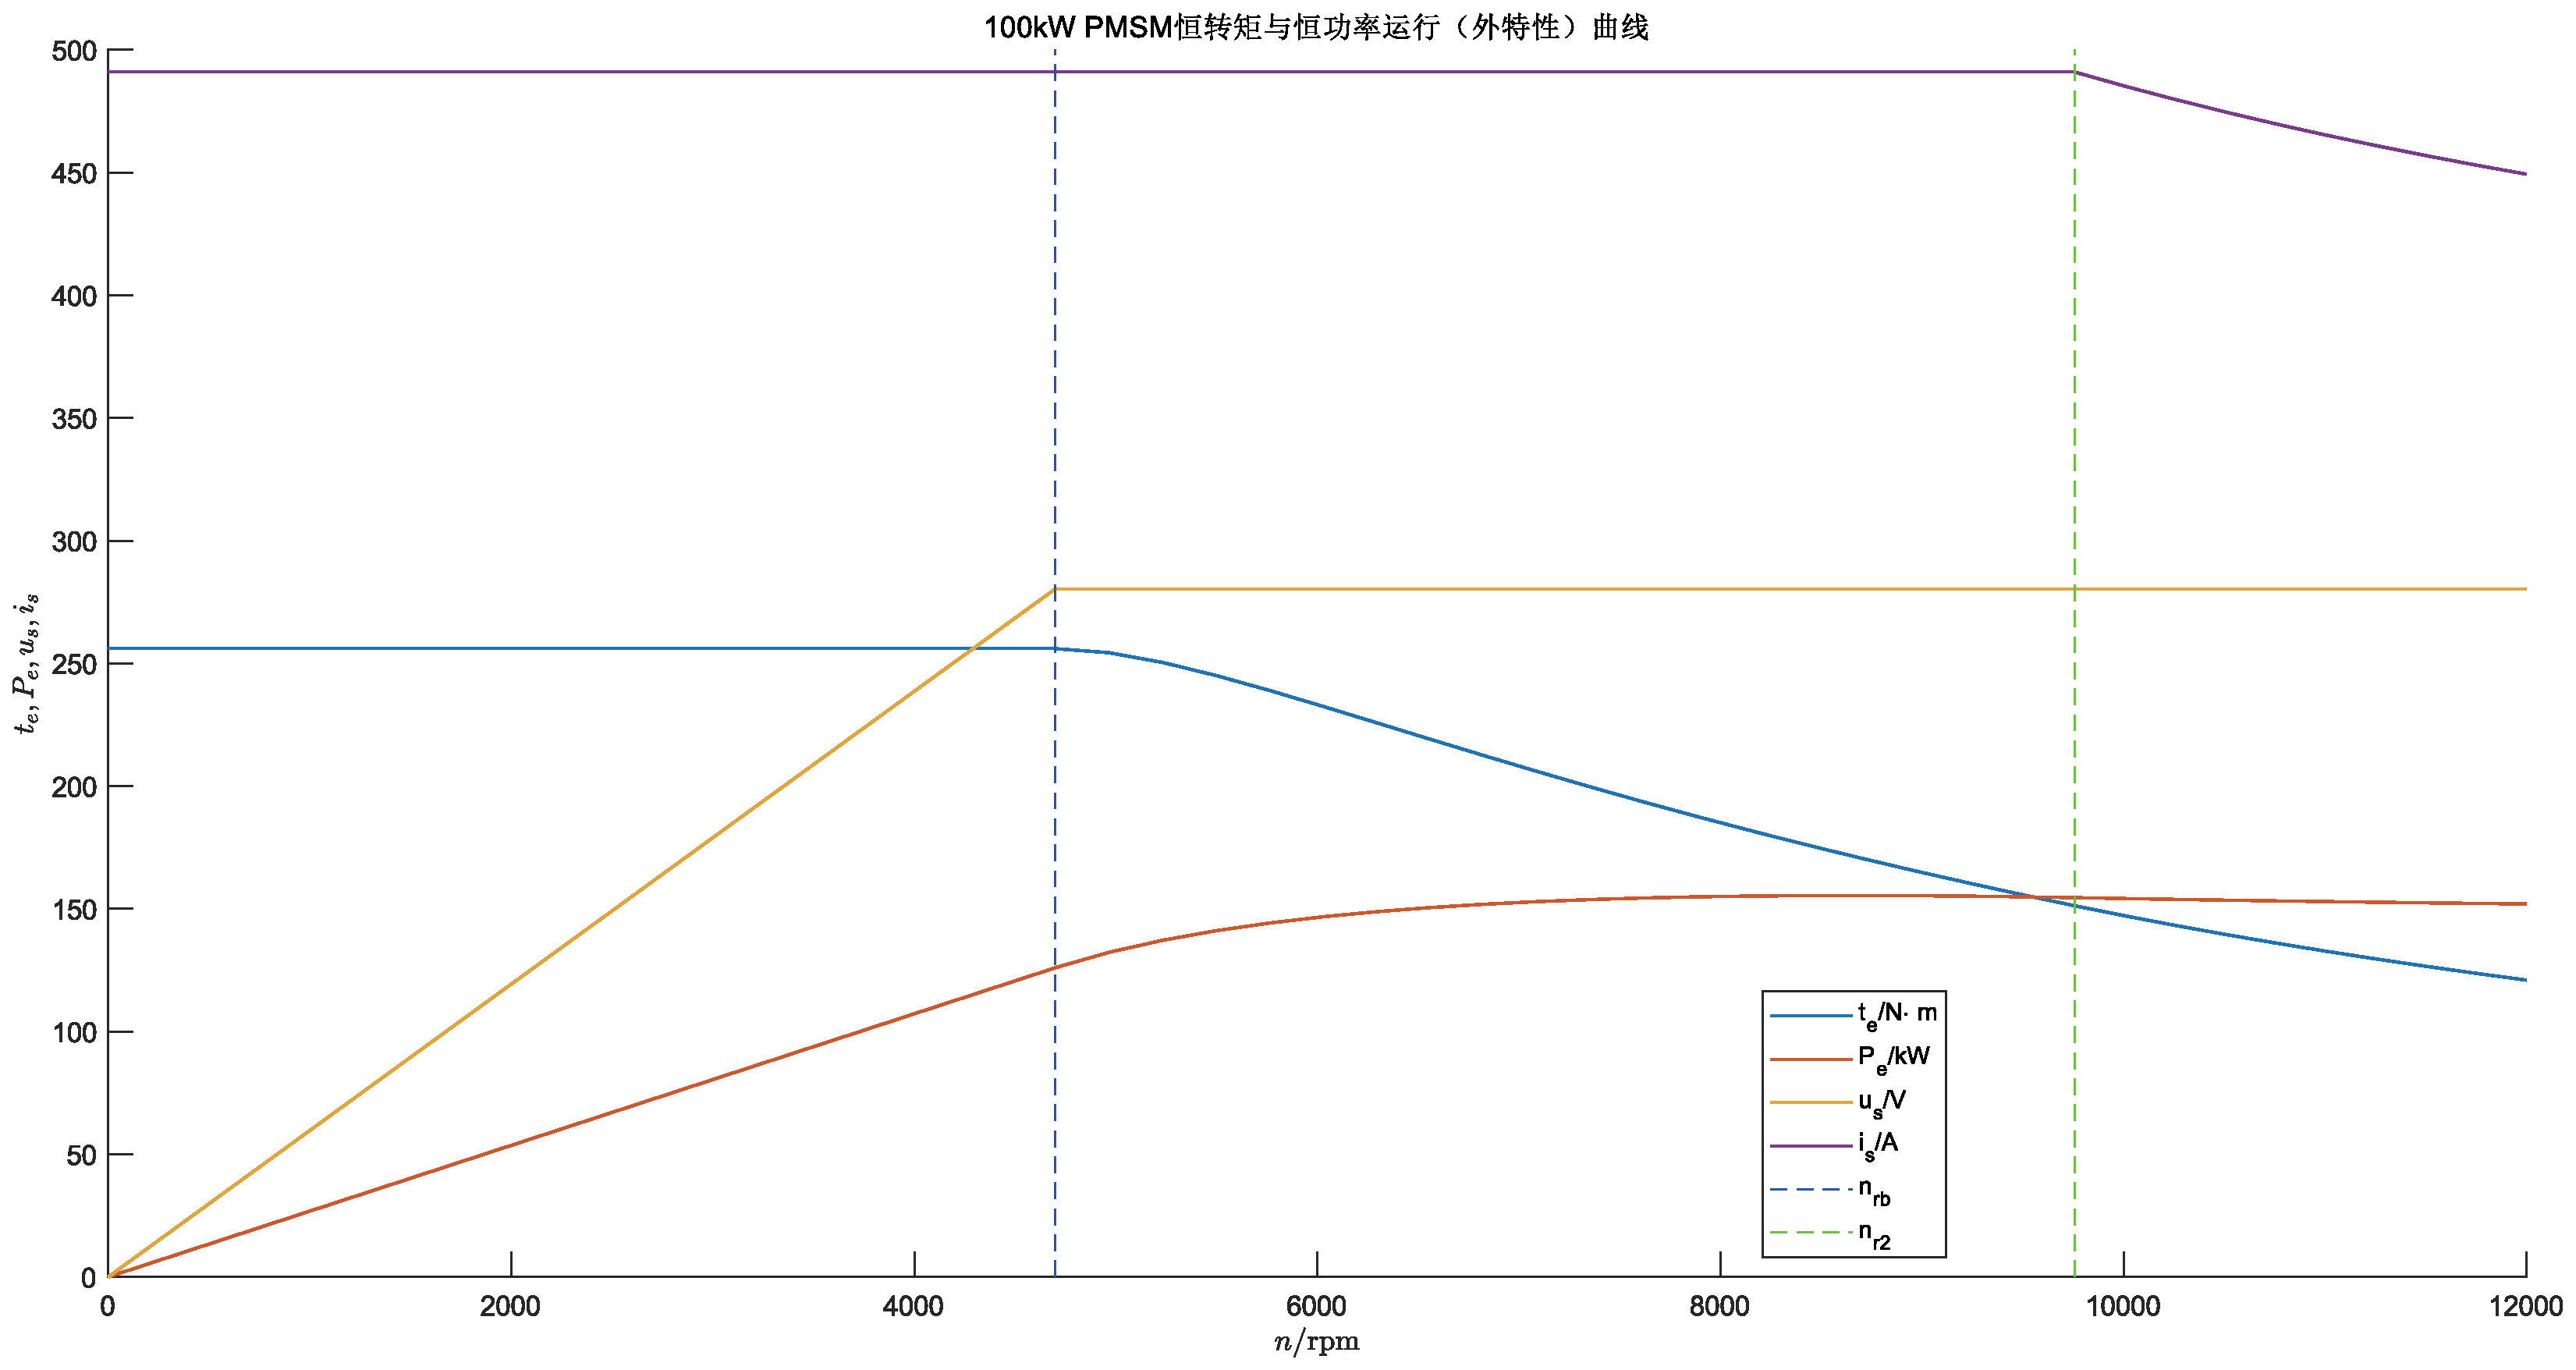
\includegraphics[width=1\textwidth]{6}
	\caption{机械特性(外特性)}
	\label{extChar}
\end{figure}

\subsection{额定转速、最大转矩工作点的空间矢量图}
\label{subsection:2.7}

定子磁链矢量$\boldsymbol{\psi}_s^{dq}$、定子电流矢量$\boldsymbol{i}_s^{dq}$和定子电压矢量$\boldsymbol{u}_s^{dq}$的合成方程由\cref{psiVec,iVec,uVec}\cite{b}给出:
\begin{align}
	\boldsymbol{\psi}_s^{dq} & =L_d i_d+\psi_f+\jmath L_q i_q \label{psiVec}                                                \\
	\boldsymbol{i}_s^{dq}    & =i_d+\jmath i_q \label{iVec}                                                                 \\
	\boldsymbol{u}_s^{dq}    & =R_s\boldsymbol{i}_s^{dq}+\jmath\omega_sL_d i_d-\omega_sL_qi_q+\boldsymbol{e}_0 \label{uVec}
\end{align}
其中$\boldsymbol{e}_0=\jmath\omega_s\psi_f$,为永磁磁链引起的运动电动势矢量。

额定转速、最大转矩工作点下,有$i_d=i_{d\rm max}$,$i_q=i_{q\rm max}$,$\omega_s=\omega_{rb}$。$i_{d\rm max}$和$i_{q\rm max}$在\cref{subsection:2.1}中给出,$\omega_{rb}$在\cref{subsection:2.3}中给出,故可画出该工况下的空间矢量图如\cref{spaceVec1}。

\begin{figure}[htbp]
	\centering
	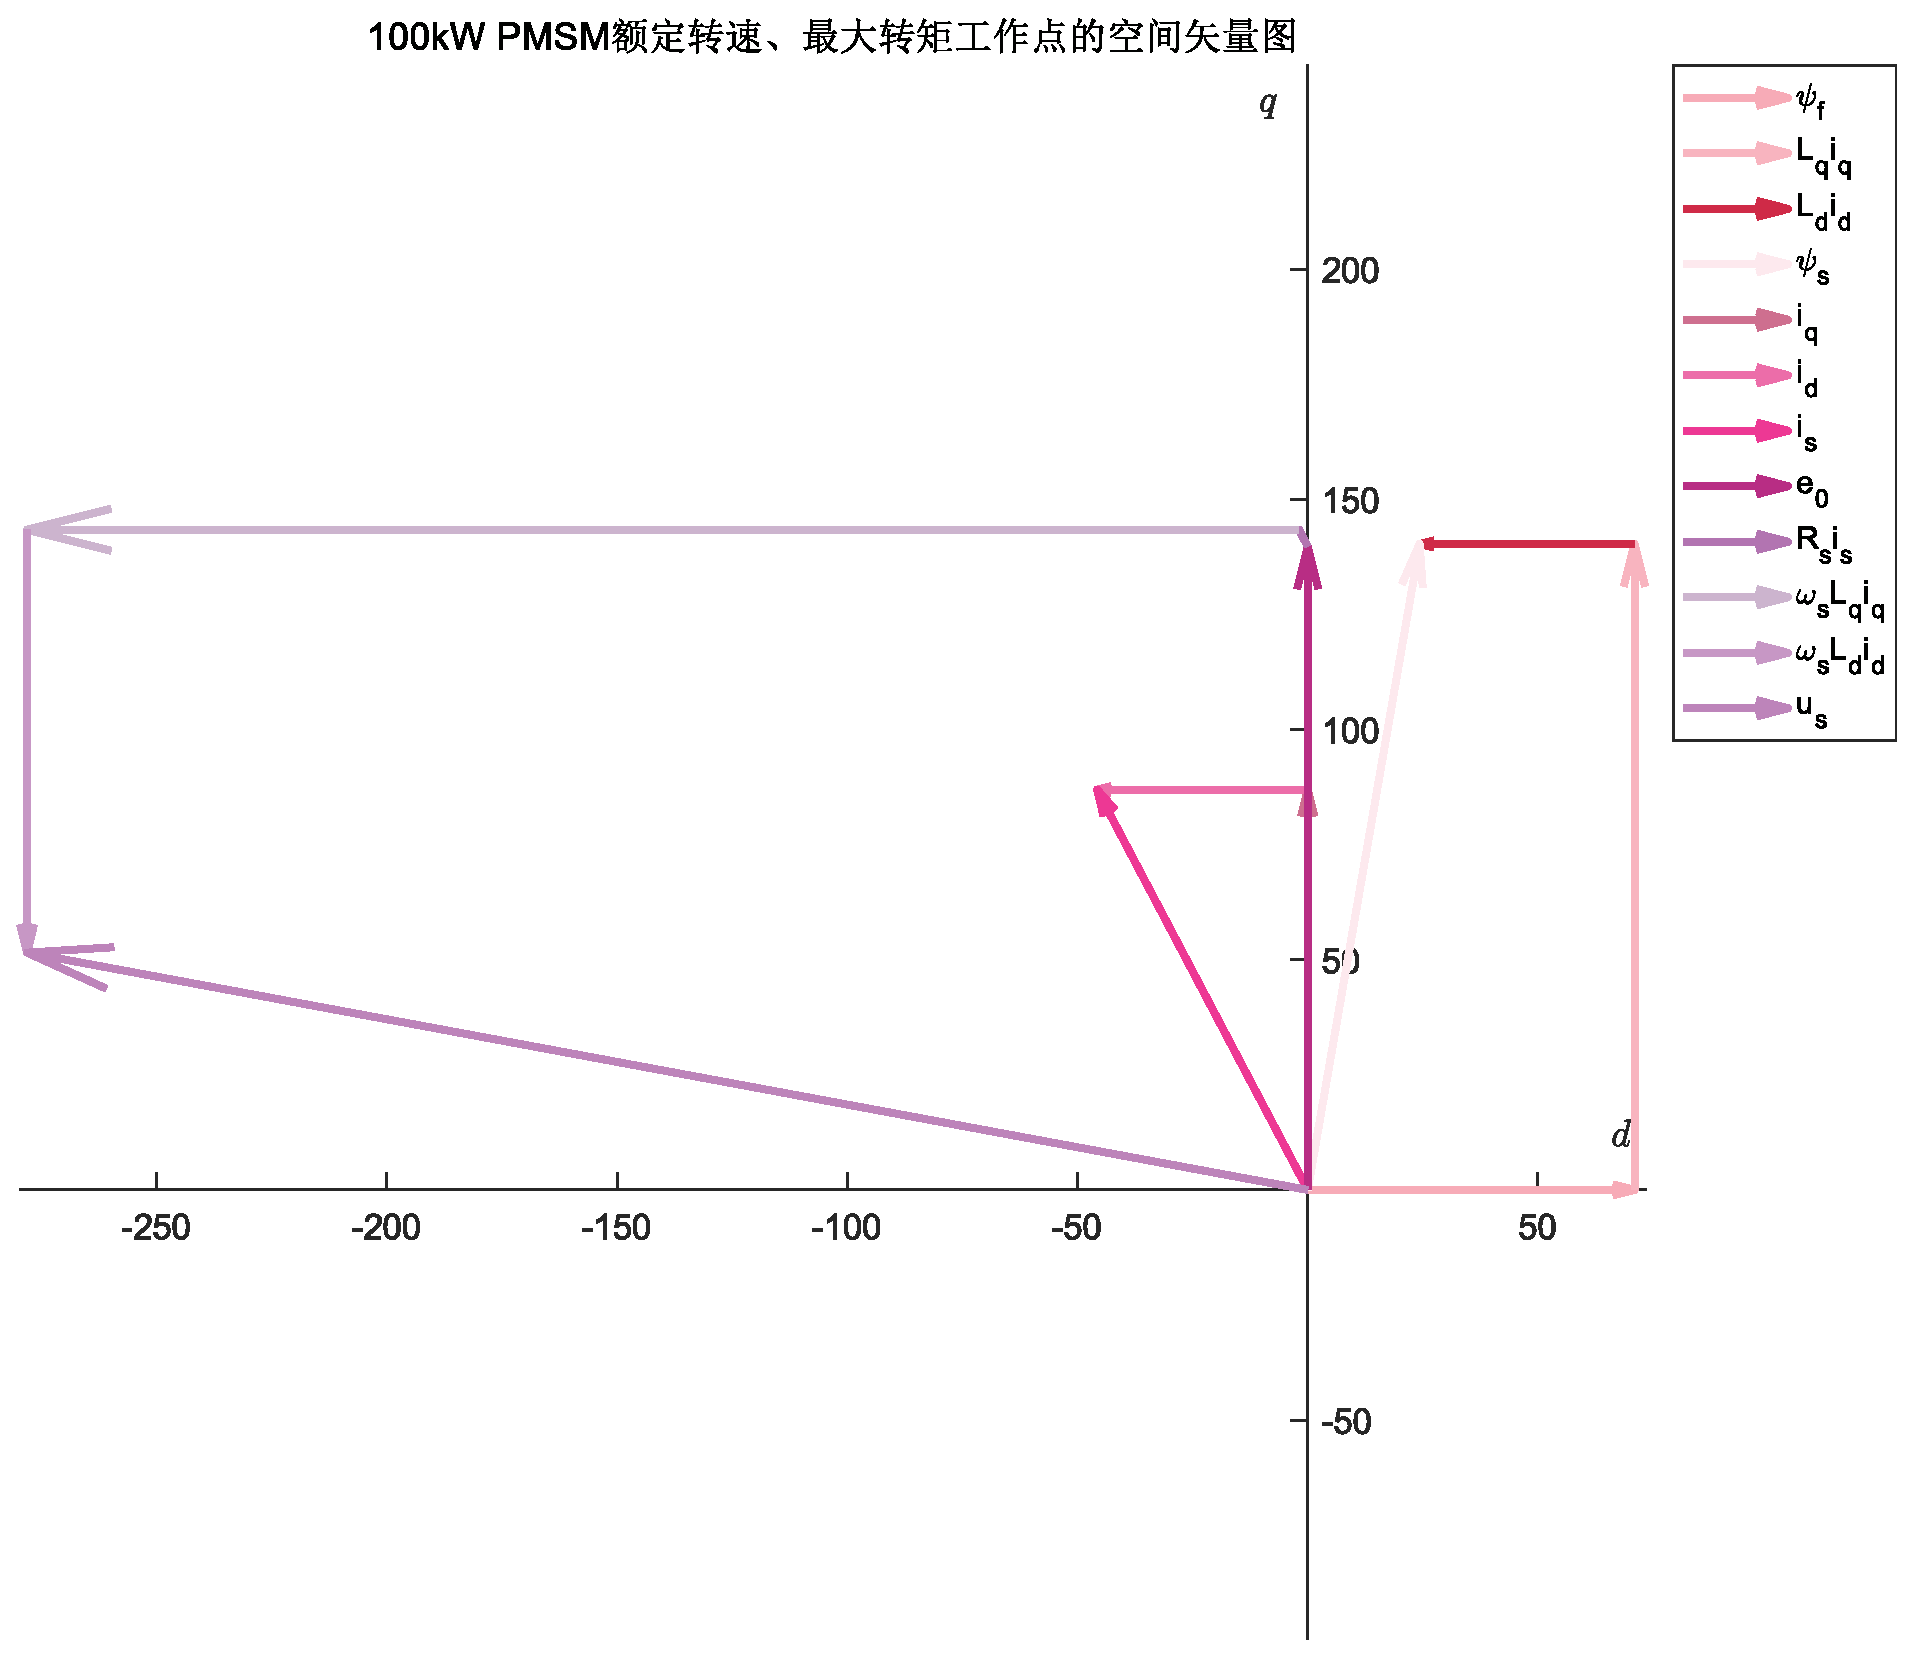
\includegraphics[width=0.8\textwidth]{7}
	\caption{额定转速、最大转矩工作点的空间矢量图}
	\label{spaceVec1}
\end{figure}

\subsection{额定转速、最大制动转矩回馈制动的空间矢量图}
\label{subsection:2.8}

根据MTPA线的对称性(\cref{MTPA,equtque}),此工况下有$i_d=i_{d\rm max}$,$i_q=-i_{q\rm max}$,$\omega_s=\omega_{rb}$,画出空间矢量图如\cref{spaceVec2}。

\begin{figure}[htbp]
	\centering
	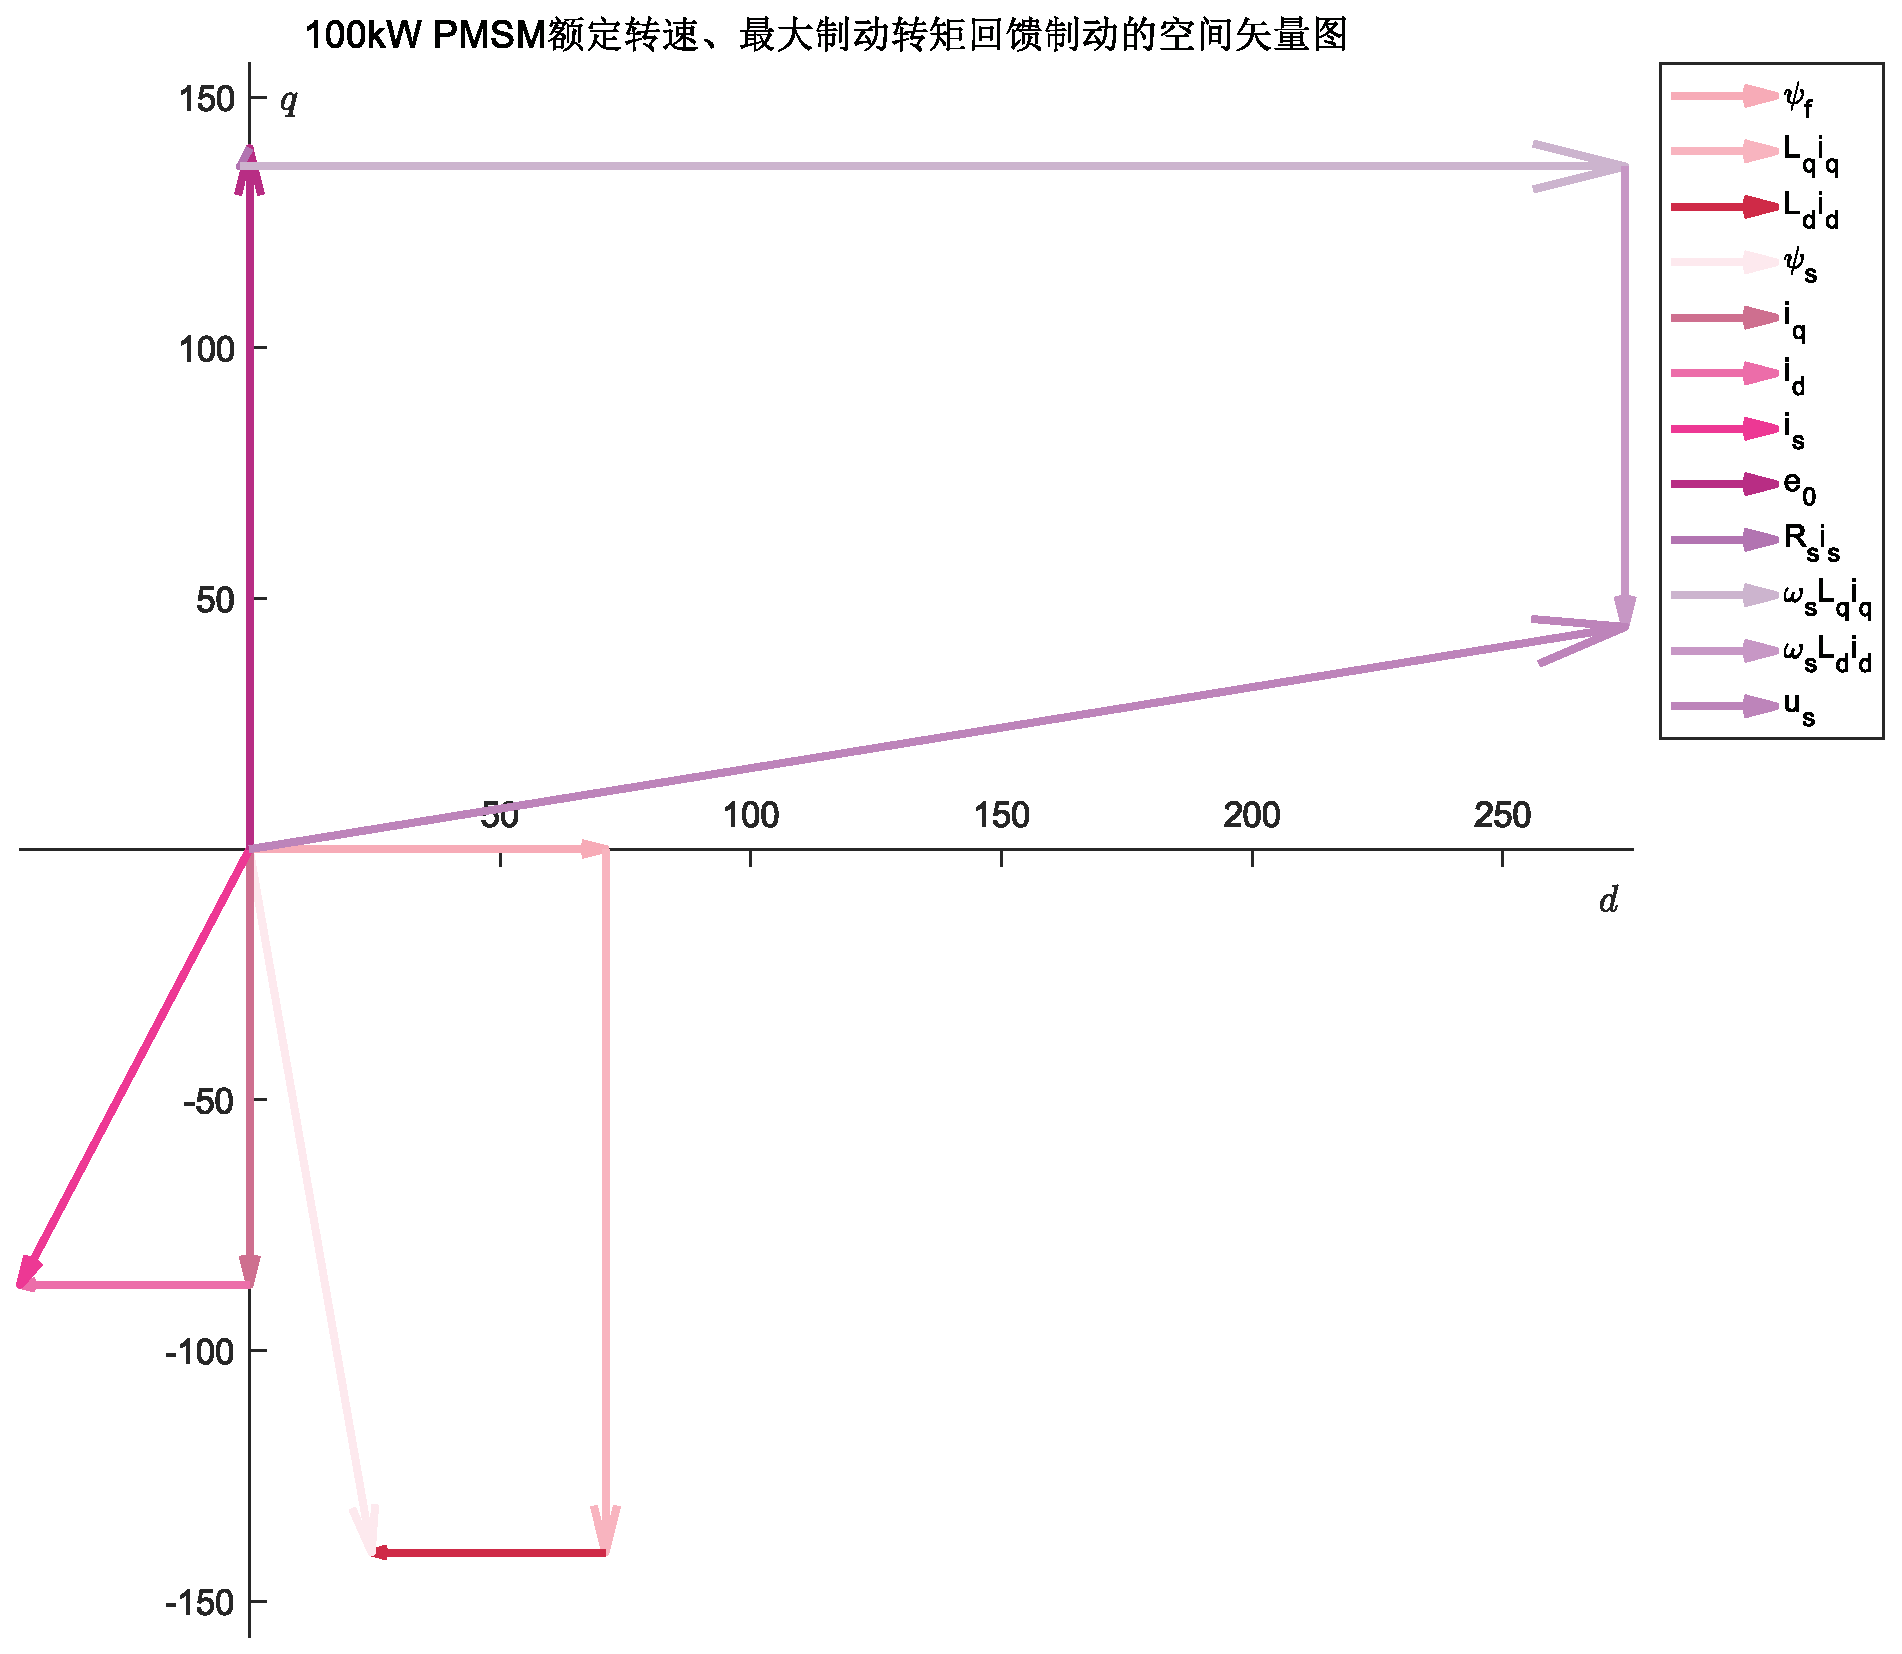
\includegraphics[width=0.8\textwidth]{8}
	\caption{额定转速、最大制动转矩回馈制动的空间矢量图}
	\label{spaceVec2}
\end{figure}

\subsection{MTPA对应的最佳电流分配曲线}
\label{subsection:2.9}

半径为$i_s$的圆和MTPA曲线在II象限的交点$(i_d,i_q)$即为每个$i_s$在最佳电流分配曲线中对应的$i_d$和$i_q$,如\cref{MTPACurDiv}。

\begin{figure}[htbp]
	\centering
	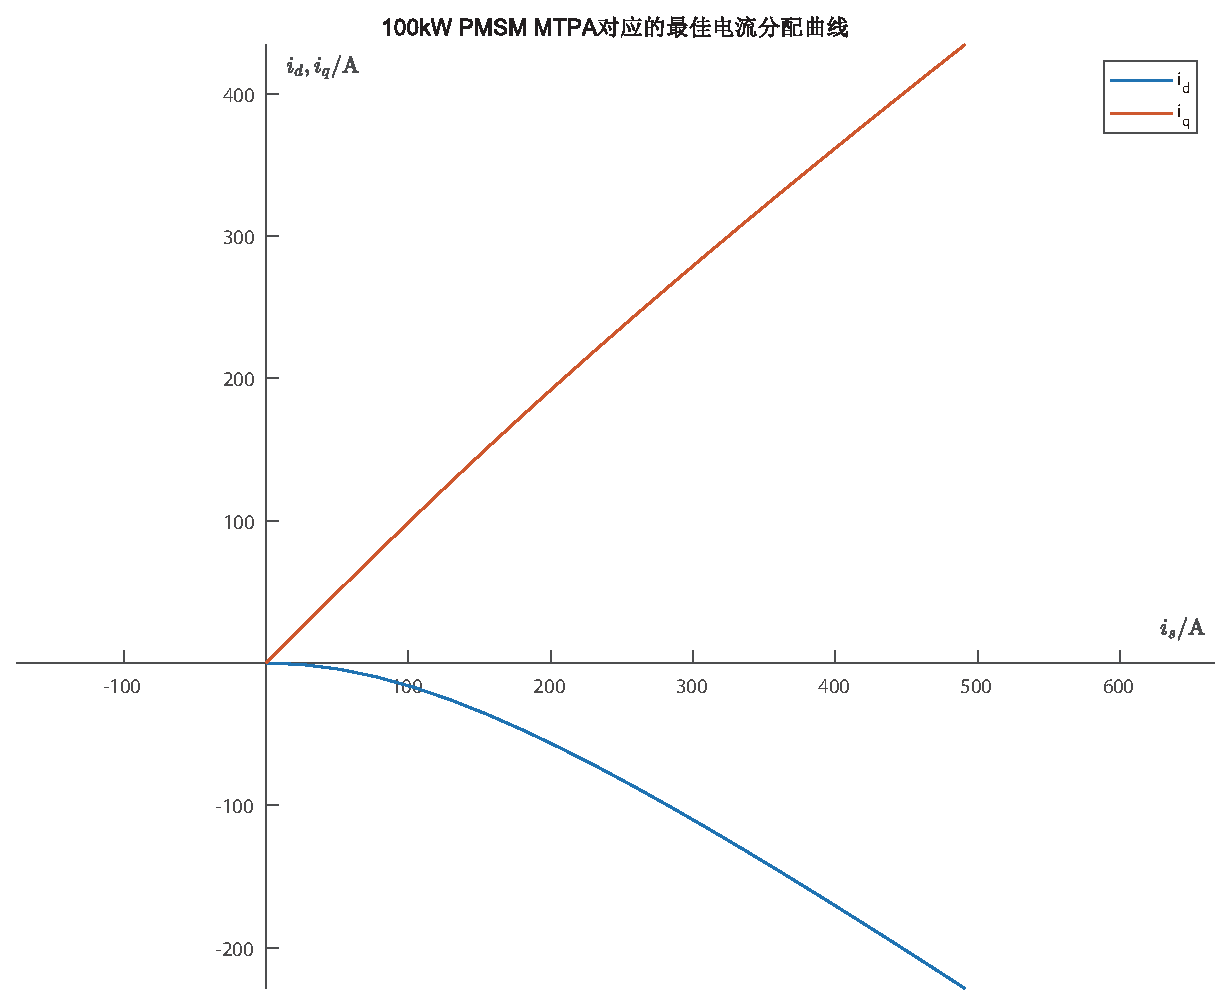
\includegraphics[width=0.8\textwidth]{9}
	\caption{MTPA对应的最佳电流分配曲线}
	\label{MTPACurDiv}
\end{figure}

\subsection{不同电流幅值下的``矩角特性曲线"}
\label{subsection:2.10}

电磁转矩$t_e$可写成定子电流$i_s$和空间相位角$\beta$的函数\cite{b}:
\begin{equation}
	t_e=\frac{3}{2}p\left[\psi_f i_s \sin{\beta}+\frac{1}{2}(L_d-L_q)i_s^2\sin{2\beta}\right]
\end{equation}

画出不同电流幅值$i_s$下的矩角特性曲线如\cref{torAng}。注意到,各曲线峰值即为$\partial t_e/\partial\beta$的点,与MTPA线(\cref{MTPA})相对应,图中用虚线标出。

\begin{figure}[htbp]
	\centering
	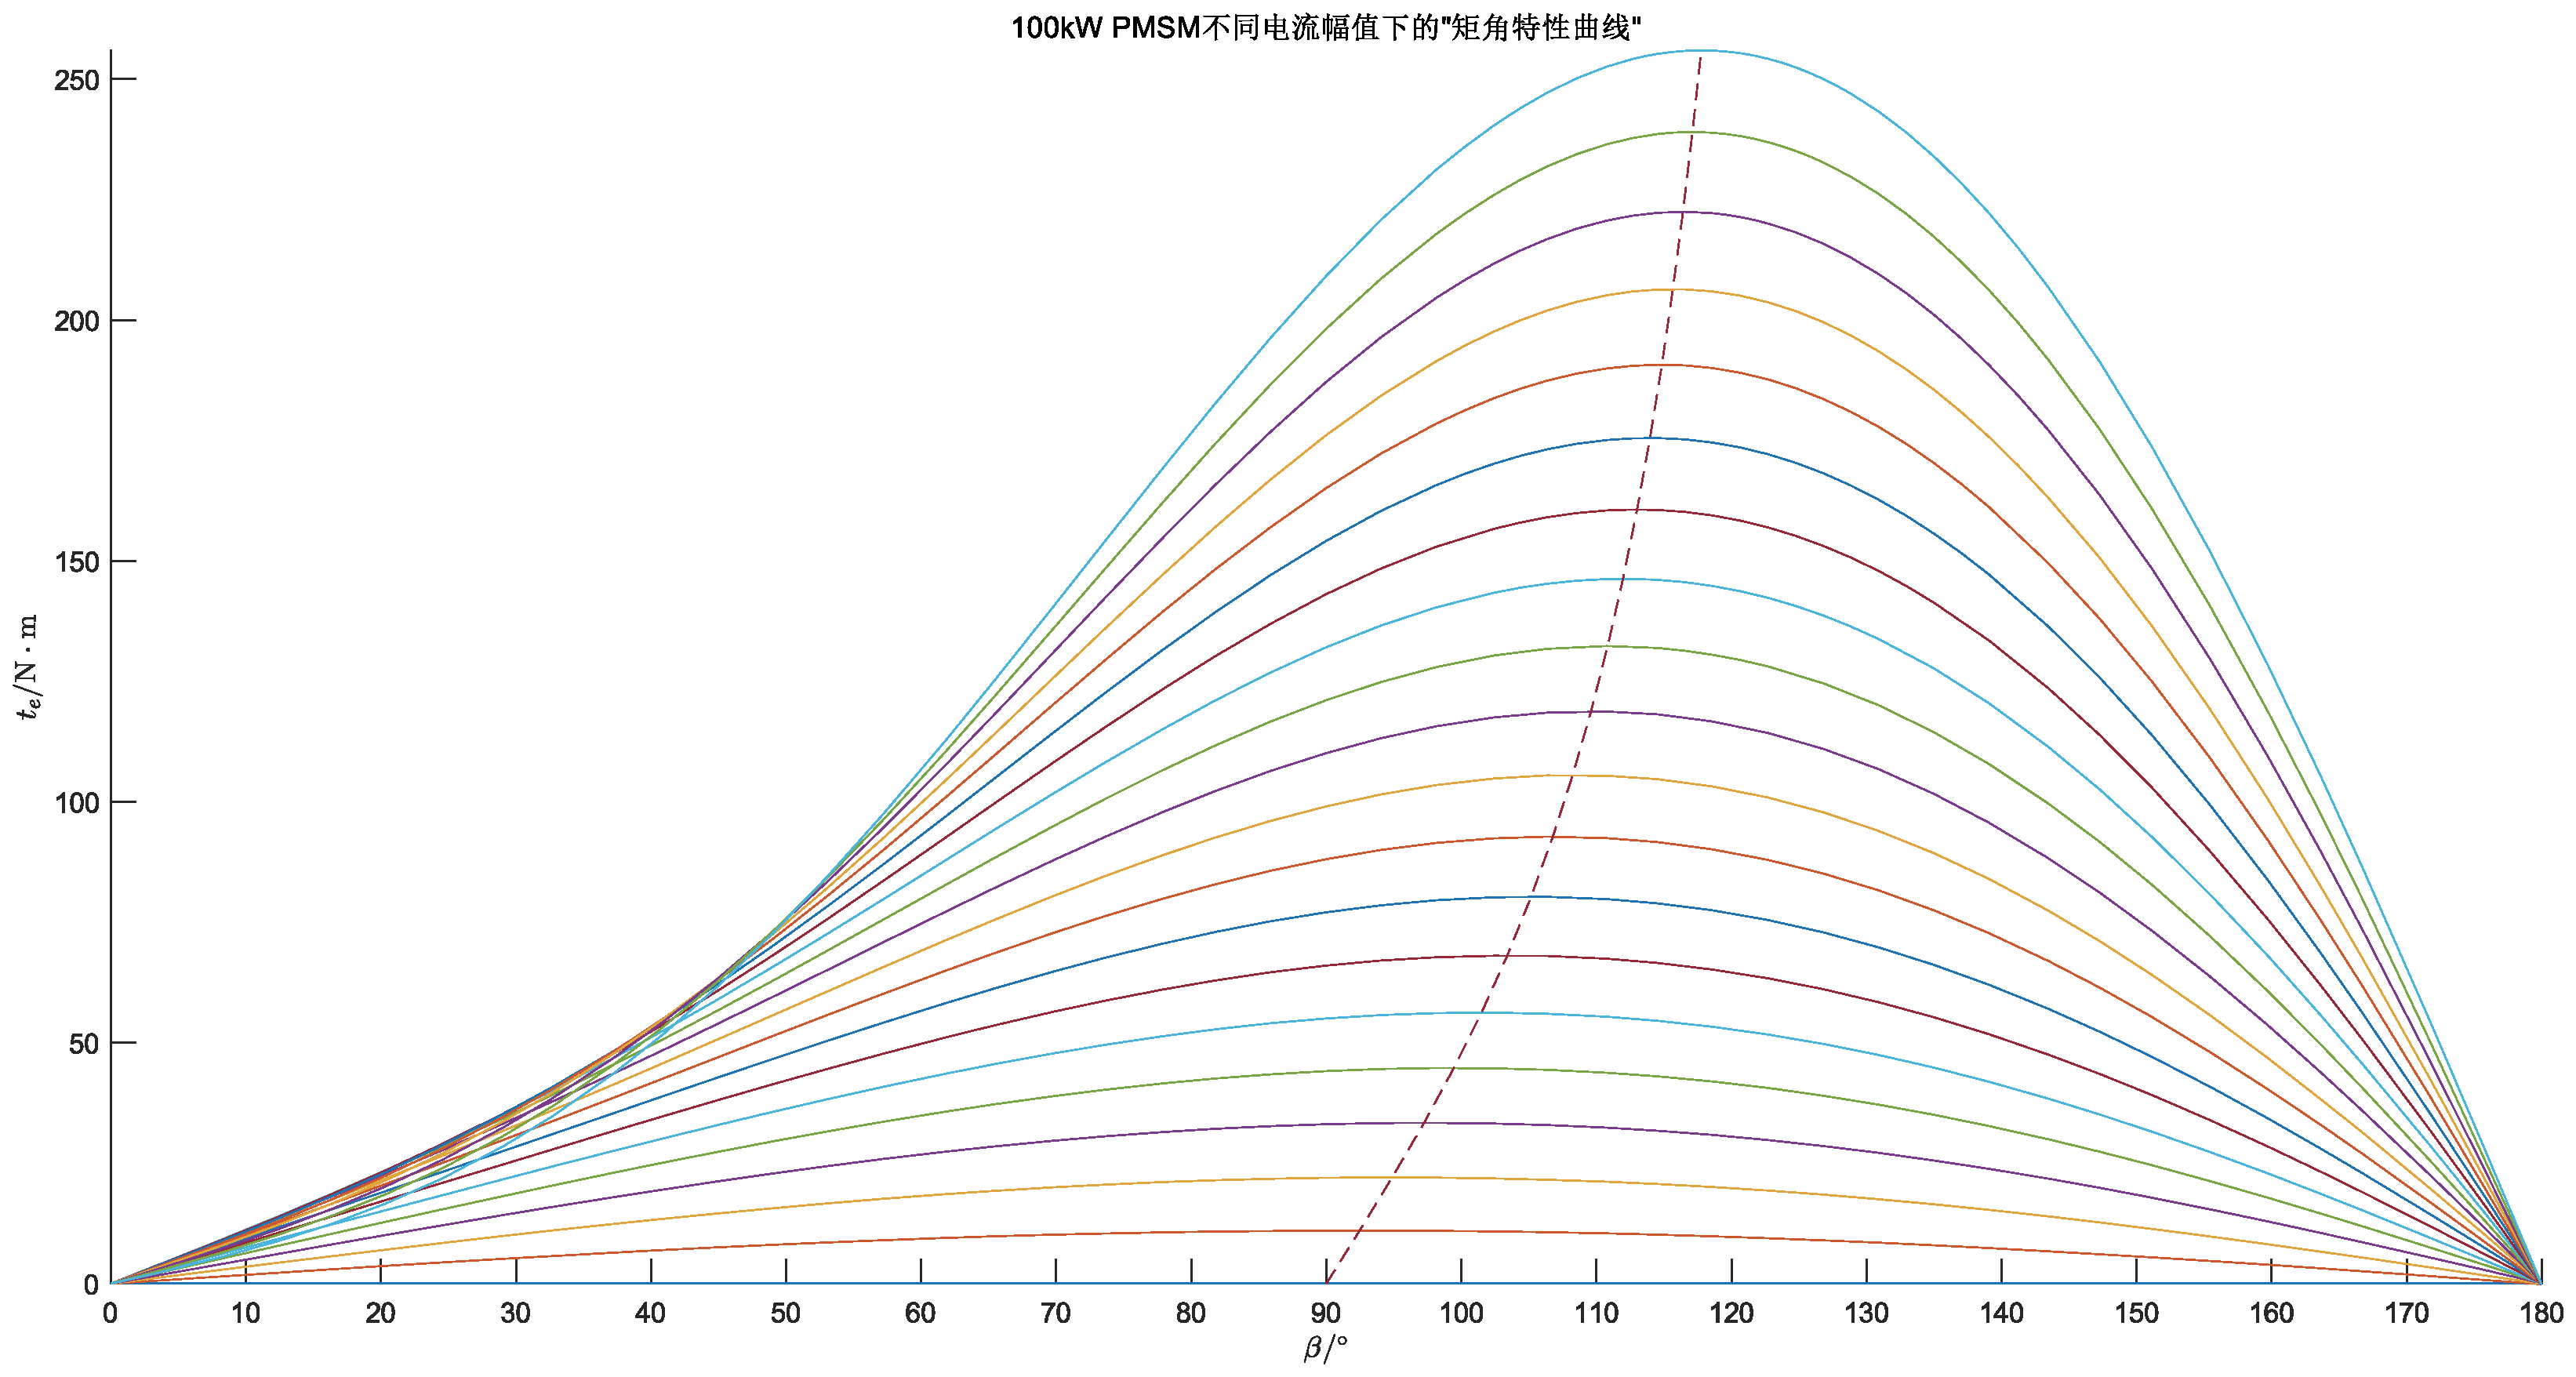
\includegraphics[width=0.8\textwidth]{10}
	\caption{不同电流幅值下的``矩角特性曲线"}
	\label{torAng}
\end{figure}

\subsection{磁阻转矩/电磁转矩曲线}
\label{subsection:2.11}

电磁转矩$t_e$由电磁转矩$t_{e\rm exci}$和磁阻转矩$t_{e\rm relu}$两部分构成,且有\cite{b}:
\begin{align}
	t_{e\rm exci} & =\frac{3}{2}p(\psi_f i_s \sin{\beta})                \\
	t_{e\rm relu} & =\frac{3}{4}p\left[(L_d-L_q)i_s^2\sin{2\beta}\right]
\end{align}

画出磁阻转矩/电磁转矩曲线如\cref{torExciReluAng}。

\begin{figure}[htbp]
	\centering
	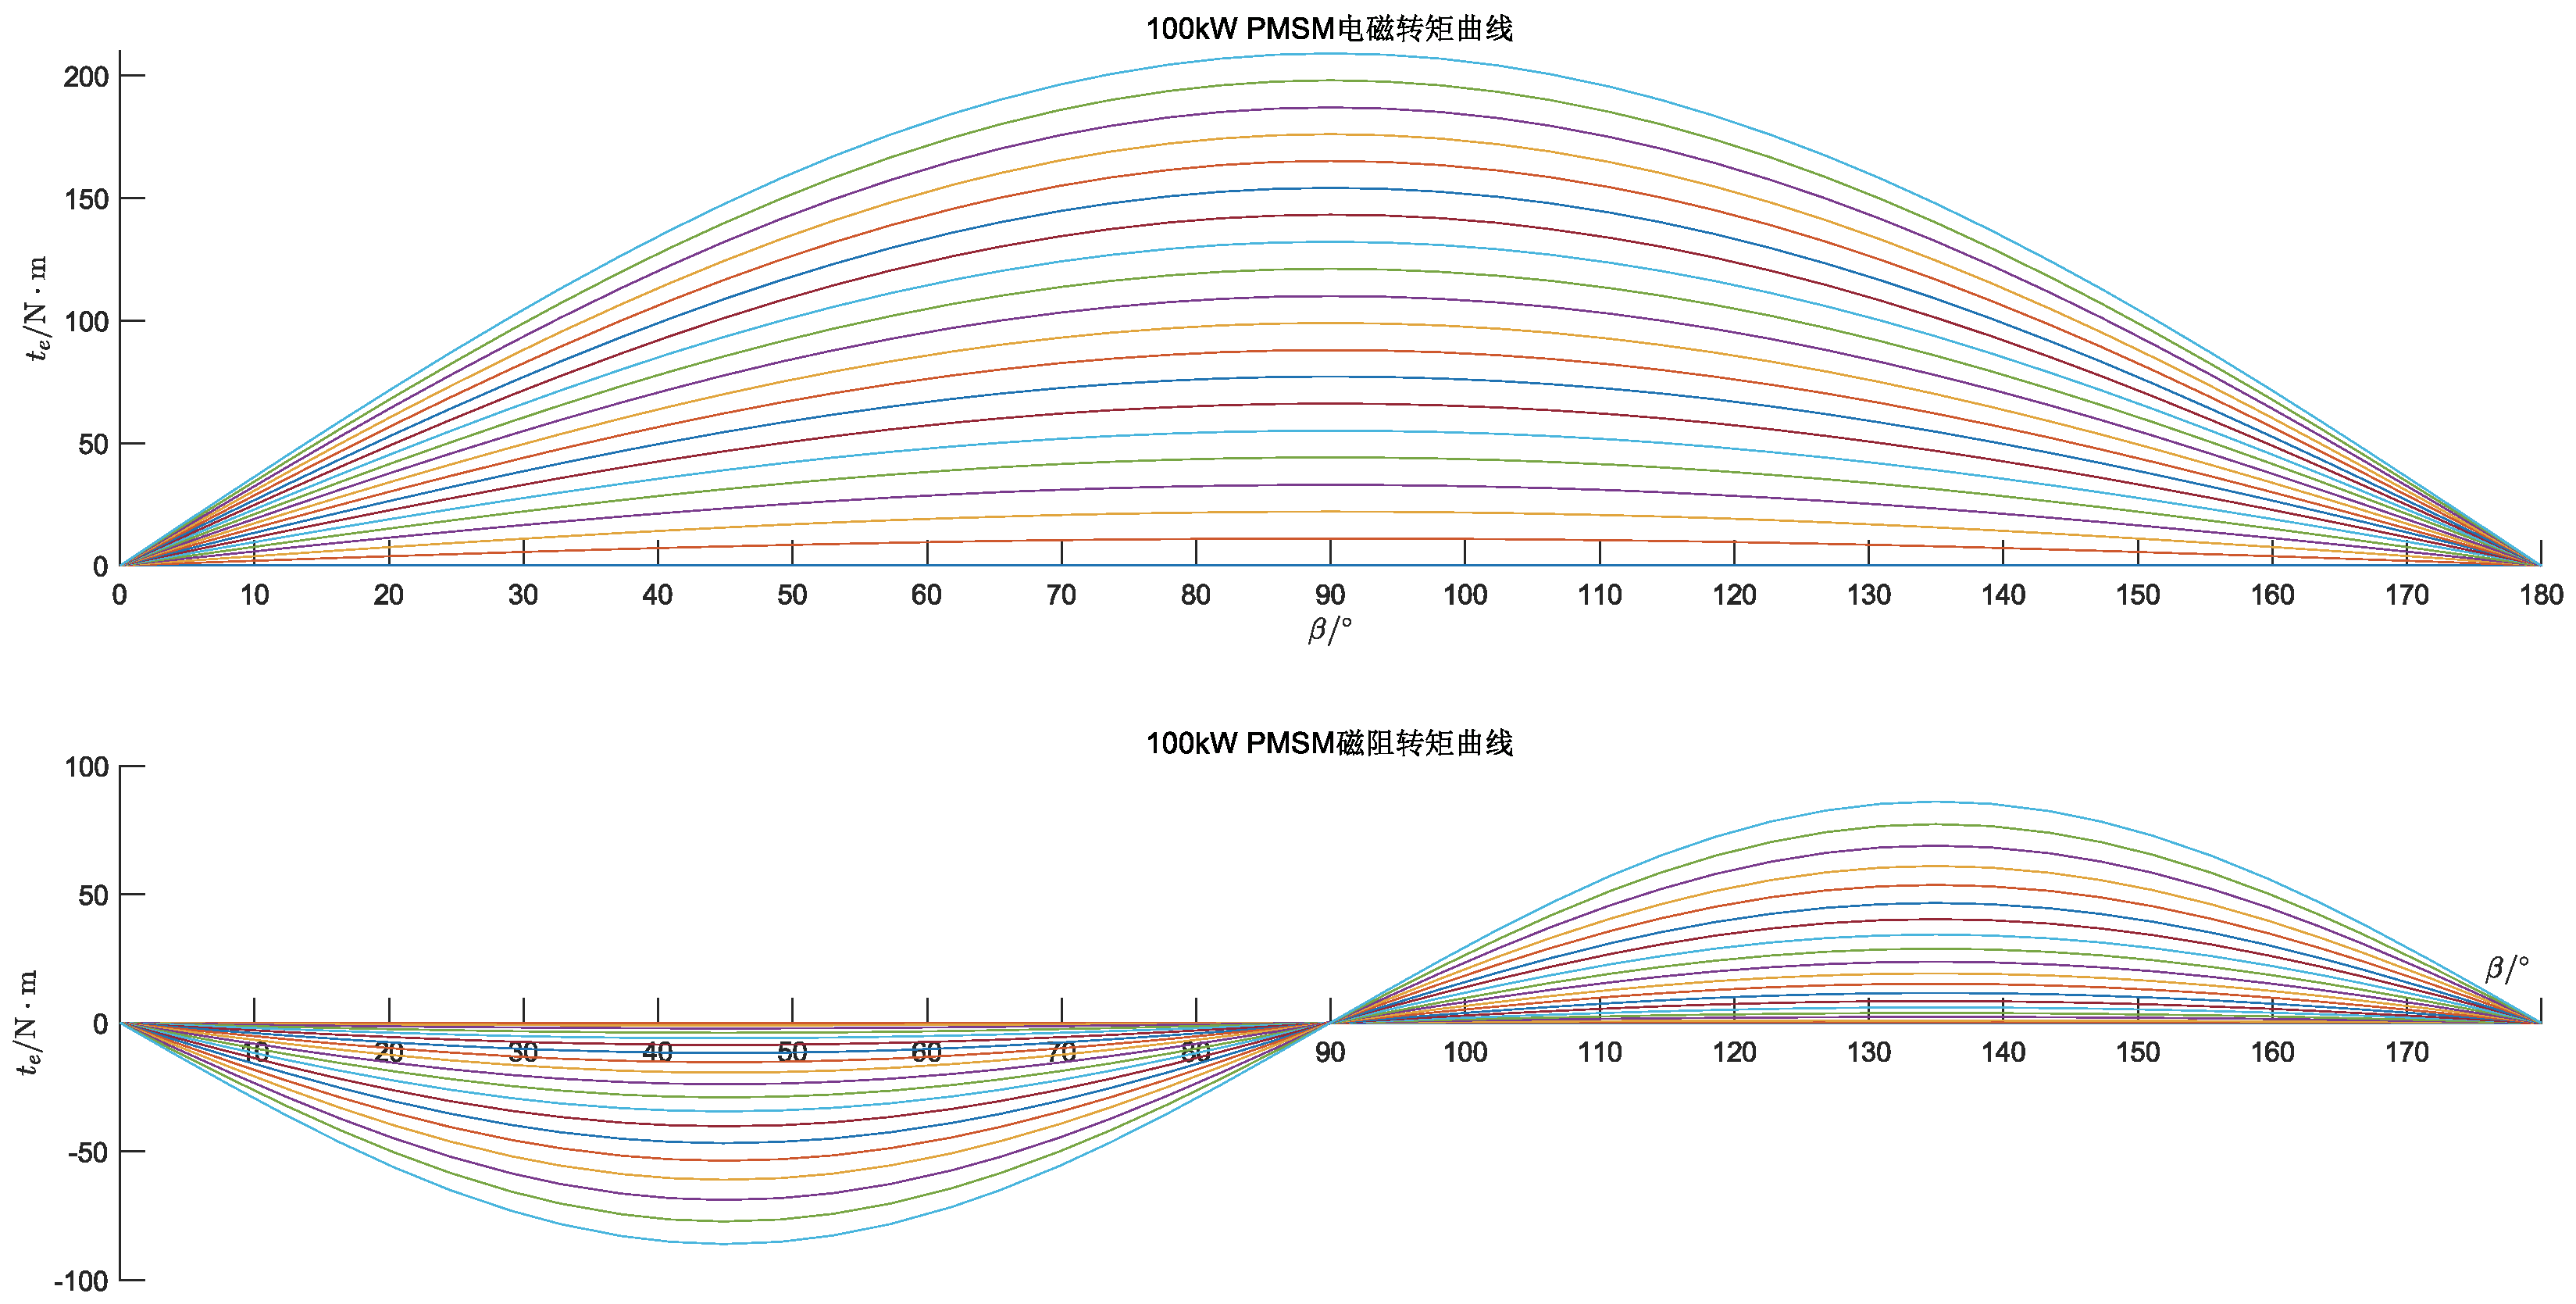
\includegraphics[width=0.8\textwidth]{11}
	\caption{磁阻转矩/电磁转矩曲线}
	\label{torExciReluAng}
\end{figure}

\clearpage

\begin{thebibliography}{99}
	\bibitem{b}钟再敏. 车用驱动电机原理与控制基础[M]. 北京:机械工业出版社, 2021.
\end{thebibliography}

\end{document}